\chapter{Loading and Storing}

Loading is the process of getting data from somewhere in the memory space into the CPU registers so that it can be used in processing. Storing is the process of getting data which is in the CPU registers into memory. Remember that seeing as flash is read-only memory, we cannot store data to flash address, but we can store to RAM.

The general format for a load is that a destination register, a register containing a base address, and an offset are supplied. An effective address is then calculated as the base address plus the offset. The contents of memory at the effective address are then copied from memory into the destination CPU register. When we do this we are treating a register as a \emph{pointer}. When we regard the contents of a register as a memory address and use that register to access data in memory we are dereferencing a pointer: accessing the data pointed to by a pointer. This is an important concept!

A store operation is very similar. Again, a register containing a base address and an offset are supplied, but this time it is a source register not a destination register which is supplied. Again, and effective address of base plus offset is calculated. The contents of the source register is copied into the effective address. 

Note that most of the load/store operations which we will be doing are 32-bit (word) load or stores. This is because the CPU registers are 32 bits. So far we have only spoken of a single effective address. As you know, each address can only hold 8 bits. Hence, in order to load or store 32 bits, four sequential addresses are used. The effective address specifies the \emph{lowest} in the sequence of the addresses. For example, if we wanted to store the contents of R0 in 0x20000000, the word would be placed into the address range 0x20000000, 0x200000001, 0x20000002 and 0x20000003. Remember that our processor uses little endian format, so the LSB is placed at 0x20000000 and the MSB at 0x20000003.

We will now explore some implementations of loading and storing.

\section{Immediate Offset Loading}
In this format, the base address is supplied in one of high CPU registers (R0 - R7), and the offset is supplied as an immediate number. 
The instruction format for loading data into a register is
\begin{lstlisting}[fontadjust=true,frame=trBL]
LDR Rt, [Rn, #imm]
\end{lstlisting}
where \texttt{Rt} is the target register for the load, \texttt{Rn} contains the base address and \texttt{\#imm} is the offset from the base address.

The way that this instruction works is that it calculates an \emph{effective address} which is equal to the contents of the base address register plus whatever number is supplied as an immediate operand.
There is, however, a slight complexity in how the offset is dealt with.

\subsection{Offset restrictions}
\label{sec:load-store-restrictions}
Remember that all instructions are limited to 16 bits. The format of the LDR instruction in machine code is shown in \autoref{fig:ldr}. We can see that after 5 bits of opcode and $2 \times 3 = 6$ bits of register specifications, we are only left with 5 bits of offset. Normally, these 5 bits would only allow us to provide an offset of $2^5 - 1 = 31$ bytes. This is not very much! In order to extend the range of the 5 offset bits, the actual offset used is equal to the 5 bit immediate number multiplied by four. This multiplication by four is the same as appending two zeros to the end of the binary value, which you can see is being done in \autoref{fig:ldr}. This means that the amount which we are able to offset a base address by is now $(2^5 - 1) \times 4 = 124$, which is significantly more useful. However, seeing as we are multiplying to immediate number by four to get the actual offset, the implication is that all offsets \emph{must} be a multiple of four. 
The compiler automatically takes care of dividing whatever offset we supply in our assembly instruction by four in order to get it to fit into the 5 bit immediate number, and the CPU then multiplies the immediate number by four to get the offset.

For example: if we wanted an offset of 12, the immediate number which would be placed in the instruction by the compiler would be 3.

\begin{figure}
\centering
\includegraphics[page=139, clip=true, trim=35mm 157mm 55mm 40mm, width=0.85\textwidth]{./DDI0419C_arm_architecture_v6m_reference_manual}
\caption{Machine Code representation of LDR instruction. Source: ARMv6-M Architecture Reference Manual}
\label{fig:ldr}
\end{figure}

\section{Program Counter Relative Loading}
There is another format of the LDR instruction which takes the Program Counter as a base register, and allows for an 8-bit immediate offset. If you wish to load data from flash into a CPU register, it makes sense to use the PC as a base register due to the fact that the PC is already initialised to be pointing to an address in flash. Specifically, it is pointing to the instruction which is being fetched (not executed - remember the three stage pipeline!). The format of the LDR instruction for PC relative loading can either be specified in the same was as the general LDR instruction, or it can have a label provided as an operand, as follows:
\begin{lstlisting}[fontadjust=true,frame=trBL]
LDR Rt, [PC, #imm]
LDR Rt, <label>
\end{lstlisting}
If one supplies a label as an operand, all that the compiler does is calculate the correct immediate offset value to insert, and compiles the instruction as if it were in the first format. It's important to note that these instructions are exactly equivalent: all that using a label does is cause the compiler to do the hard work of calculating the correct offset so you don't have to. It would really be a lot of hard work; every time you changed something in the structure of your program which caused instructions to be moved to different memory addresses (like writing a new line of code!) you'd potentially have to re-calculate your offsets. The ability to use labels is one of the most useful features of the compiler.


\section{Register Offset Loading}
So far all offsets have been supplied as immediate numbers to the load instructions. However, there is another format of the load instruction called a register-offset load. Here, the offset is contained in another register. This is useful as the offset can be set at run-time by modifying the contents of a register, rather than at compile time. In this case, the effective address is calculated as the contents of the base register (\texttt{Rn}) plus the contents of the offset register (\texttt{Rm}). 
\begin{lstlisting}[fontadjust=true,frame=trBL]
LDR Rt, [Rn, Rm]
\end{lstlisting}

\section{Storing}
The storing commands are so similar to the loading that they will barely be discussed. One difference is that there is no PC-relative store, as there would be no point trying to store data to read-only memory. The store instruction takes moves the contents of a source register, \texttt{Rt}, and places it at the effective memory address equal to the base address, \texttt{Rn}, plus an offset either supplied as a 5-bit immediate number, \texttt{\#imm5}, or in an offset register, \texttt{Rm}.

\begin{lstlisting}[fontadjust=true,frame=trBL]
STR Rt, [Rn, #imm5]
STR Rt, [Rn, Rm]
\end{lstlisting}

\section{Accessing of Datatypes Other Than Words}
So far we have only loaded or stored words. While it is useful to be able to move an entire 32 bits of data around at once we will sometimes only want to move bytes of half-words around. There are instructions which allow us to do this. There is a version of the \texttt{LDR} instruction which loads only 1 byte: \texttt{LDRB}. Similarly, there is a version which loads 2 bytes or half a word: \texttt{LDRH}. 
